\chapter{Combatants}

\begin{table}[ht!]
\begin{small}
\rowcolors{2}{}{commentgreen}
\begin{center}
\begin{tabular}{ccccl}
\multicolumn{5}{l}{\parbox[l][0.6cm][c]{15cm}{\textbf{The Combatant}}} 
\\
\hline 
\textbf{Level} & \textbf{Prof} & \textbf{Stamina} & \textbf{Points} & \parbox[l][0.6cm][c]{11cm}{\textbf{Features}} 
\\ 
1st & +2 & 1d6 & 2 & \parbox[l][0.6cm][c]{11cm}{Fighting Style, Path feature}
\\
2nd & +2 & 1d6 & 3 & \parbox[l][0.6cm][c]{11cm}{Extra feat}
\\
3rd & +2 & 1d8 & 3 & \parbox[l][0.6cm][c]{11cm}{Path feature}
\\
4th & +2 & 1d8 & 3 & \parbox[l][0.6cm][c]{11cm}{Extra feat, Ability Score Improvement}
\\
5th & +3 & 1d8 & 4 & \parbox[l][0.6cm][c]{11cm}{Extra Attack}
\\
6th & +3 & 1d8 & 4 & \parbox[l][0.6cm][c]{11cm}{Extra feat}
\\
7th & +3 & 1d8 & 4 & \parbox[l][0.6cm][c]{11cm}{Indomitable, Path feature}
\\
8th & +3 & 1d8 & 5 & \parbox[l][0.6cm][c]{11cm}{Extra feat, Ability Score Improvement}
\\
9th & +4 & 1d10 & 5 & \parbox[l][0.6cm][c]{11cm}{Path feature}
\\
10th & +4 & 1d10 & 5 & \parbox[l][0.6cm][c]{11cm}{Extra feat}
\\

\hline
\end{tabular}
\end{center}
\end{small}
\end{table}

\begin{multicols*}{2}

\section*{Class Features} 

As a combatant, you gain the following class features.

\textbf{Hit Dice:} 1d10

\textbf{Hit Points at 1st Level:} 14 + your Constitution modifier

\textbf{Hit Points at Higher Levels:} 4 + your Constitution modifier per fighter level after 1st


\textbf{Armor:} All armor, shields

\textbf{Weapons:} Simple weapons, martial weapons

\textbf{Saving Throws:} Strength, Constitution

\textbf{Skills:} Choose two skills from Acrobatics, Animal Handling, Athletics, History, Insight, Intimidation, Medicine, Perception, and Survival 
    
\section*{Stamina} 

You have a poll of stamina dices to use. A common use of your stamina is to enhance an attack in some way. Each path specializes on the usage of stamina in a different way. For example, a fighter has controlled fighting maneuvers while a barbarian uses stamina to endure attacks.



\begin{itemize}
    \item You regain all stamina points when finish a short or long rest.
    \item You regain 1 stamina point whenever an enemy scores a critical hit against you;
    \item You regain 1 stamina point whenever an ally within sight is knocked unconscious;
    \item You regain 2 stamina points when you get bloodied.
\end{itemize}

Outside of combat, you can use stamina to double you jump distance, gain a stamina die bonus to any athletics roll, or hold a collapsing portal, tunnel, wall, etc. for your stamina die minutes.

   
\section*{Extra Attack} 

Beginning at 5th level, you can attack twice, instead of once, whenever you take the Attack action on your turn.


\section*{Fighting Style}

You adopt a particular style of fighting as your specialty. Choose one of the following options. You can’t take a Fighting Style option more than once, even if you later get to choose again.


\begin{itemize}
    \item Archery You gain a +1 bonus to attack rolls you make with ranged weapons.
    \item Defense While you are wearing armor, you gain a +1 bonus to AC. 
    \item Dueling When you are wielding a melee weapon in one hand and no other weapons, you gain a +2 bonus to damage rolls with that weapon.
    \item GWF When you roll a 1 or 2 on a damage die for an attack you make with a melee weapon that you are wielding with two hands, you can reroll the die and must use the new roll, even if the new roll is a 1 or a 2. The weapon must have the two-handed or versatile property for you to gain this benefit. 
    \item TWF When you engage in two-weapon fighting, you can add your ability modifier to the damage of the second attack.
\end{itemize}


\begin{Figure}
\centering
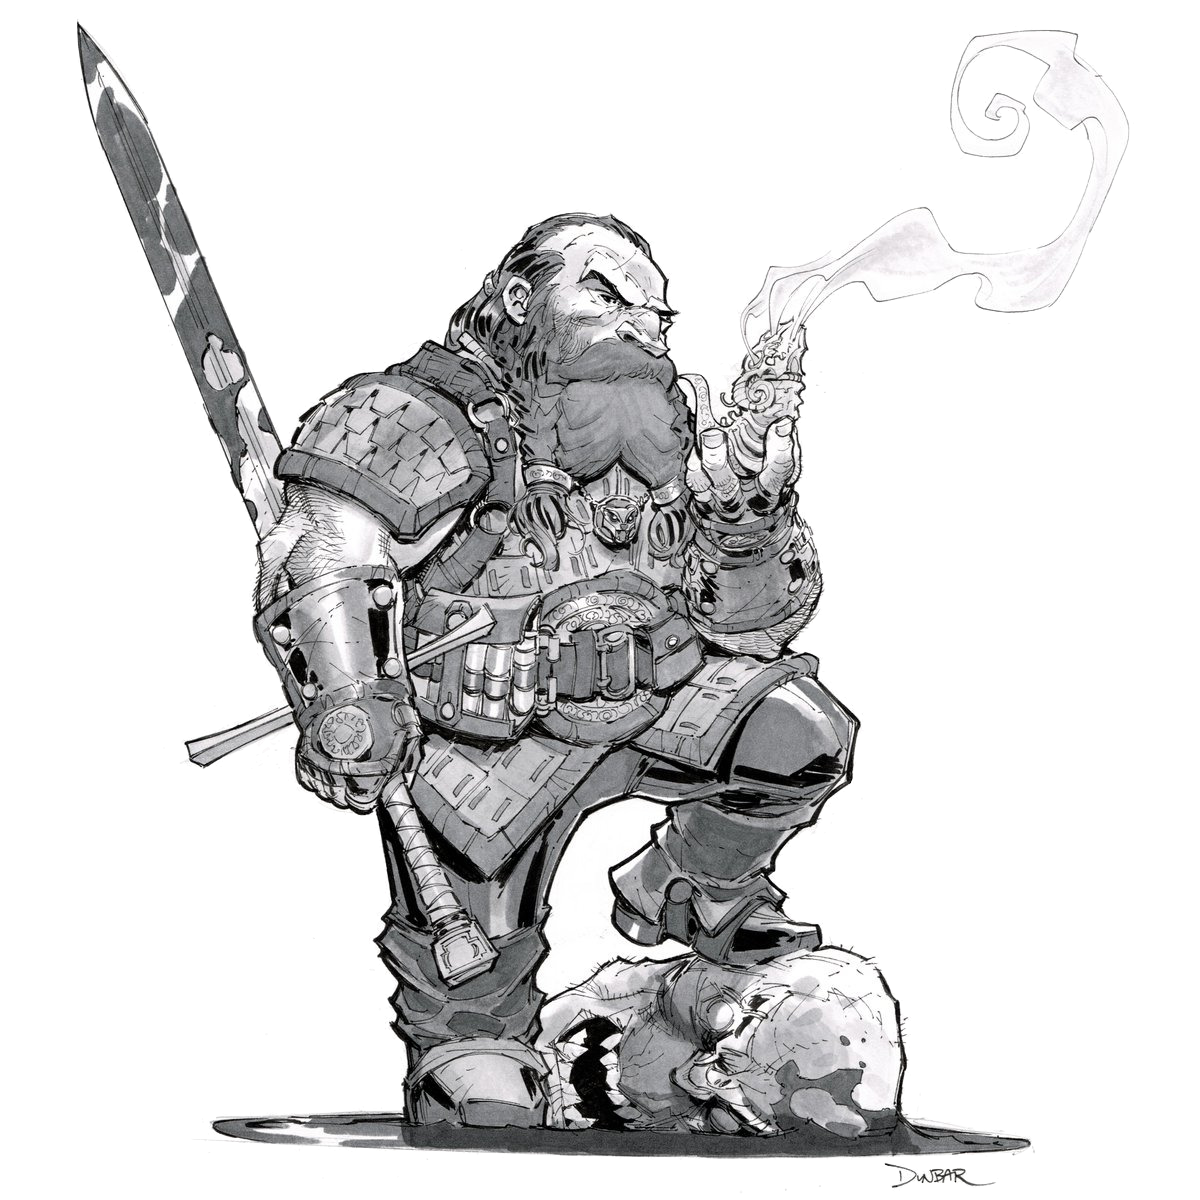
\includegraphics[width=\textwidth]{img/fighter-dwarf.png}
\end{Figure}
    

\section*{Indomitable}

Beginning at 7th level, you can reroll a saving throw that you fail. If you do so, you must use the new roll, and you can’t use this feature again until you finish a long rest.




\end{multicols*}

\clearpage


\begin{multicols*}{2}



\section{Barbarian}

\lettrine[lines=3, lhang=0.15, loversize=0.25, findent=.5em]{B}{arbarians} are tired of the empty battles they once craved. They wander, outcast, while their tribes curse the gods who abandoned them. They are consumed with rage and longing for foes worthy of their rage.

\subsection*{Rage}

In battle, you fight with primal ferocity. Starting at 1st level, on your turn, you can use one point of stamina to enter a rage as a bonus action.



While raging, you gain the following stats if you aren’t wearing heavy armor:


\begin{itemize}
    \item You have advantage on Strength checks and Strength saving throws.
    \item When you make a melee weapon attack using Strength, you gain +2 bonus to the damage roll. 
    \item You have resistance to bludgeoning, piercing, and slashing damage.
    \item If you are able to cast spells, you can’t cast them or concentrate on them while raging.
\end{itemize}

Your rage lasts for 5 turns. It ends early if you are knocked unconscious. You can also end your rage on your turn as a bonus action.



\subsection*{The Beast Within}

\subsection*{Feral Instinct}

By 7th level, your instincts are so honed that you have advantage on initiative rolls.

Additionally, if you are surprised at the beginning of combat and aren’t incapacitated, you can act normally on your first turn, but only if you enter your rage before doing anything else on that turn.

\subsection*{Relentless}

Starting at 9th level, your rage can keep you fighting despite grievous wounds. If you drop to 0 hit points while you’re raging and don’t die outright, you can make a DC 10 Constitution saving throw. If you succeed, you drop to 1 hit point instead.

Each time you use this feature after the first, the DC increases by 5. When you finish a short or long rest, the DC resets to 10.


\begin{Figure}
\centering
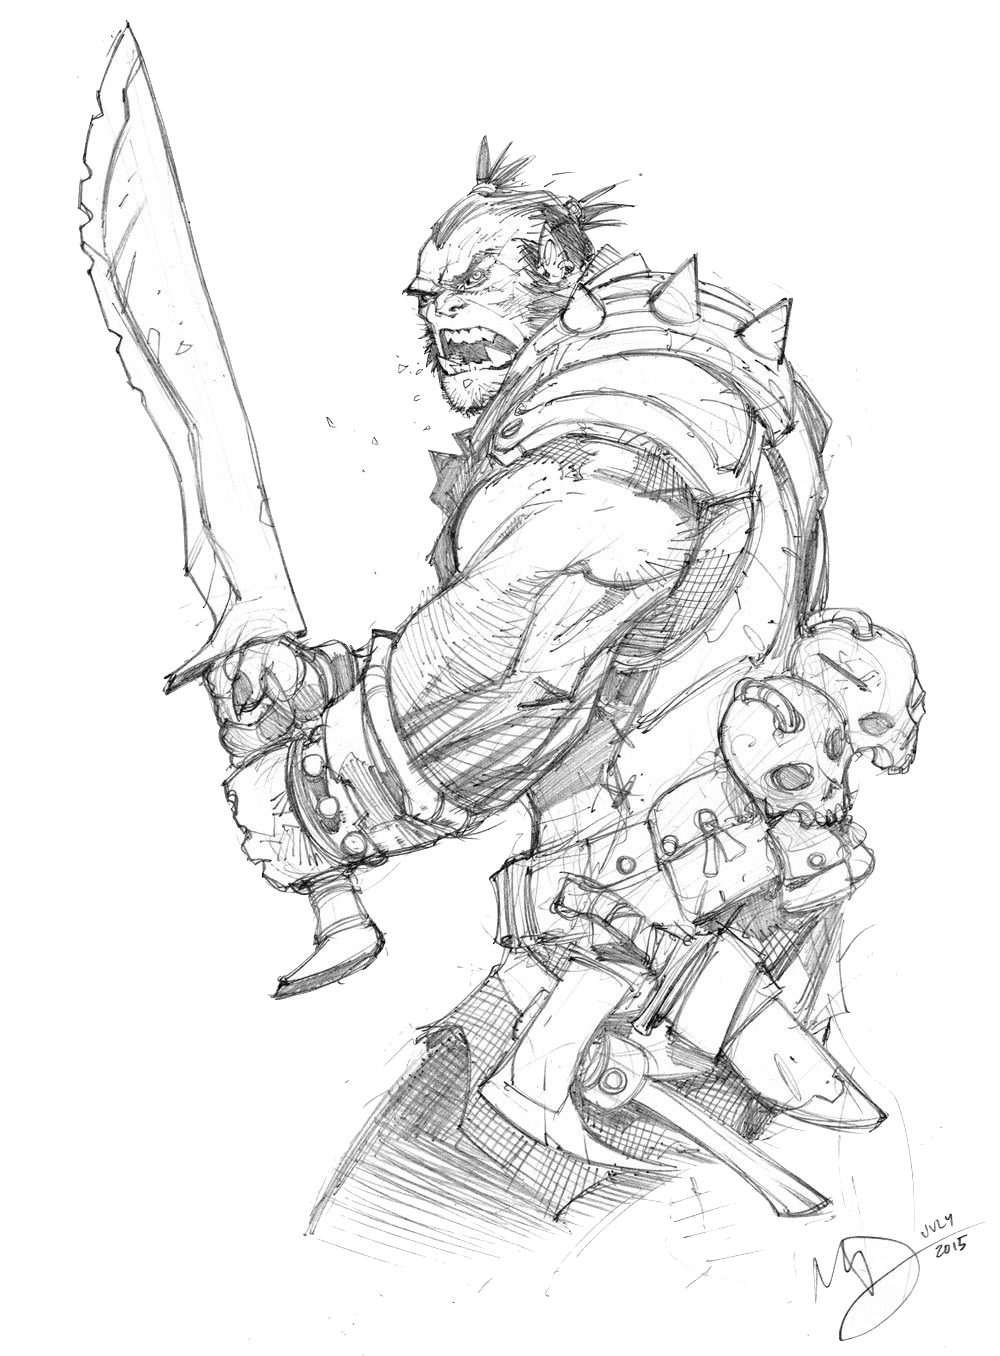
\includegraphics[width=\textwidth]{img/barbarian-half-orc.png}
{\scriptsize Art by Max Dunbar}
\end{Figure}
    
\end{multicols*}


\begin{multicols*}{2}

\section{Fighter}

\subsection*{Action Surge}

Once per turn, you can use one point of stamina to make on additional attack.



\subsection*{Maneuvers}

At 3rd level, you learn maneuvers that are fueled by your stamina dice.
You learn four maneuvers of your choice. You learn two additional maneuvers of your choice at 7th and 10th level. Note that some maneuvers require you to be holding certain weapons or carrying a shield. Refer to the  fighter's maneuvers table for descriptions.

\textbf{Saving Throws.} Some of your maneuvers require your target to make a saving throw to resist the maneuver's effects. The saving throw DC is calculated as follows:

\textbf{Maneuver save DC} = 8 + your proficiency bonus + your Strength or Dexterity modifier (your choice)

\begin{Figure}
\centering
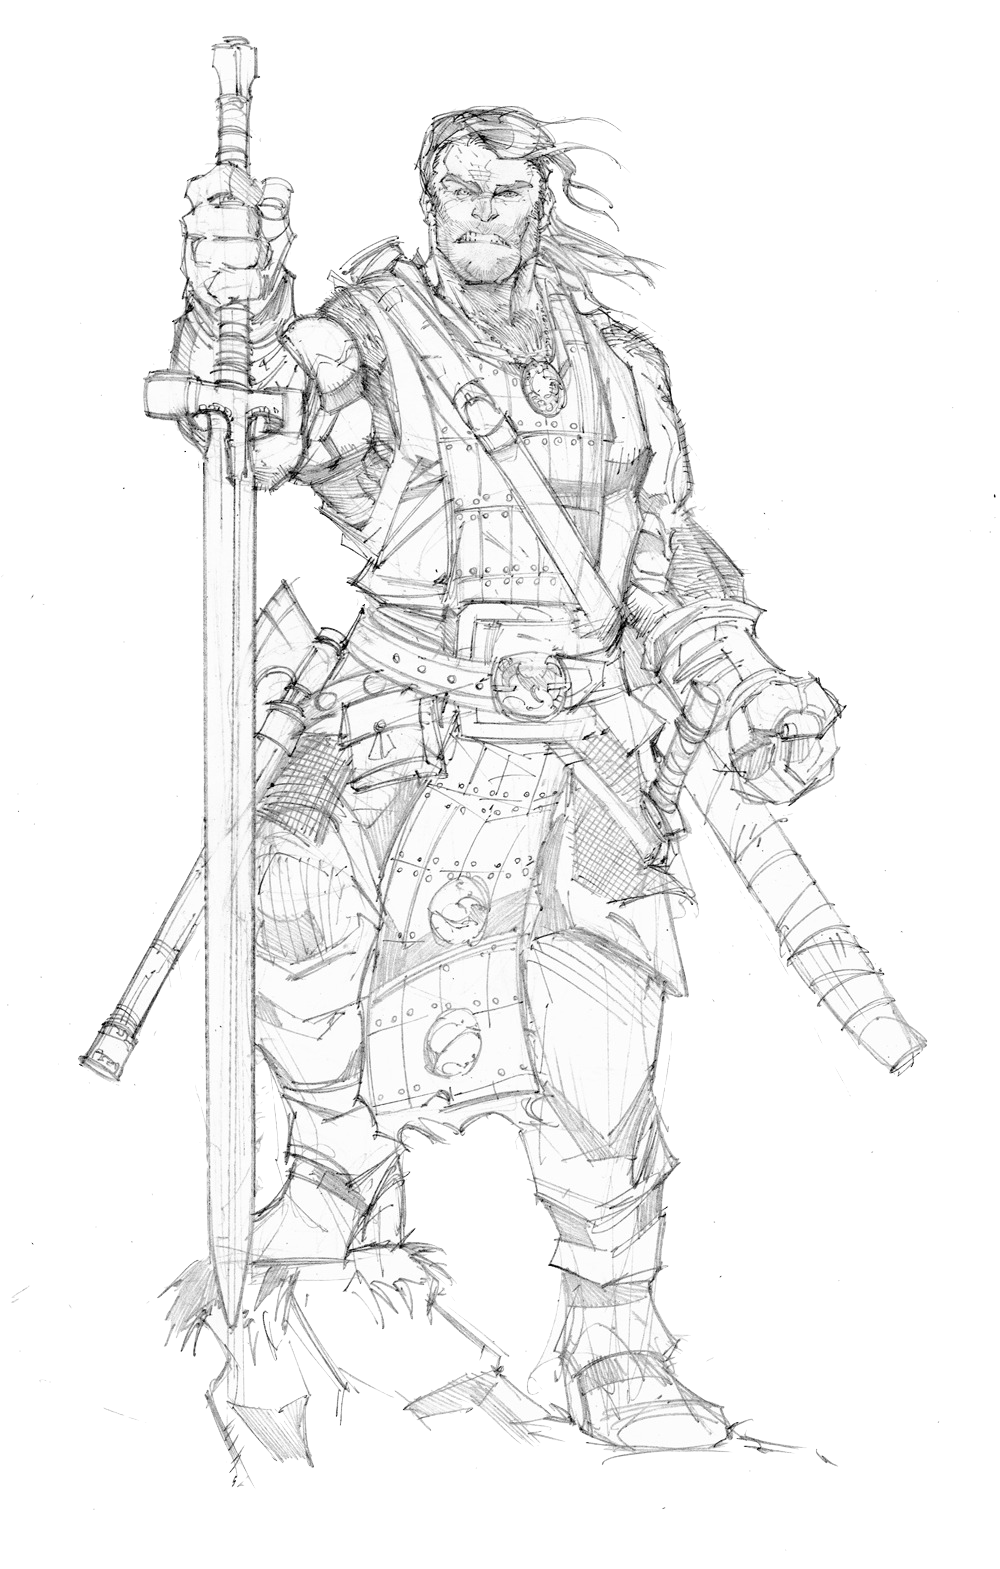
\includegraphics[width=\textwidth]{img/fighter.png}
\end{Figure}

\subsection*{War Shout}

You yell battle orders inspiring your allies. 
As a bonus action, up to three creatures within 60 feet of you including yourself gain 10 temporary hit points.
You regain one stamina point.

\subsection*{Fighting Spirit}

Your intensity in battle can shield you and help you strike true. 
When you are reduced to 0 hit points but not killed outright, you can drop to 1 hit point instead and regain 2 stamina points.

Once you use this feature, you can’t use it again until you finish a long rest.

\end{multicols*}    

\clearpage

\begin{table}[ht!]
\begin{small}
\rowcolors{2}{}{commentgreen}
\begin{center}
\begin{tabular}{ll}
\multicolumn{2}{l}{\parbox[l][0.6cm][c]{15cm}{\textbf{Fighter Maneuvers}}} 
\\
\hline 
\textbf{Name} & \parbox[l][0.6cm][c]{15cm}{\textbf{Description}}
\\ 
Goading Attack & \parbox[l][2.4cm][c]{15cm}{
When you hit a creature with a weapon attack, you can expend one stamina point to attempt to goad the target into attacking you. You add the stamina die to the attack's damage roll, and the target must make a Wisdom saving throw. On a failed save, the target has disadvantage on all attack rolls against targets other than you until the end of your next turn.
}
\\
Lunging Attack & \parbox[l][1.8cm][c]{15cm}{
When you make a melee \hl{two-handed} weapon attack on your turn, you can expend one stamina point to increase your reach for that attack by 5 feet. If you hit, you add the stamina die to the attack's damage roll.
}
\\
Maneuvering Attack & \parbox[l][2.4cm][c]{15cm}{
When you hit a creature with a \hl{reach} weapon attack, you can expend one stamina point to maneuver one of your comrades into a more advantageous position. You add the stamina die to the attack's damage roll, and you choose a friendly creature who can see or hear you. That creature can use its reaction to move up to half its speed without provoking opportunity attacks from the target of your attack.
}
\\
Menacing Attack & \parbox[l][2.1cm][c]{15cm}{
When you hit a creature with a weapon attack, you can expend one stamina point to attempt to frighten the target. You add the stamina die to the attack's damage roll, and the target must make a Wisdom saving throw. On a failed save, it is frightened of you until the end of your next turn.
}
\\
Pushing Attack & \parbox[l][2.2cm][c]{15cm}{
When you hit a creature with a \hl{bludgeoning} weapon attack, you can expend one stamina point to attempt to drive the target back. You add the stamina die to the attack's damage roll, and if the target is Large or smaller, it must make a Strength saving throw. On a failed save, you push the target up to 15 feet away from you.
}
\\
Trip Attack & \parbox[l][2cm][c]{15cm}{
When you hit a creature with a weapon attack, you can expend one stamina point to attempt to knock the target down. You add the stamina die to the attack's damage roll, and if the target is Large or smaller, it must make a Strength saving throw. On a failed save, you knock the target prone.
}
\\
Hold the Line & \parbox[l][2.8cm][c]{15cm}{
As a reaction when a hostile creature moves adjacent to an ally within 20 feet of you, you can spend one stamina point to immediately move up to your movement speed towards the creature. If you end your movement adjacent to the creature, make a Strength (Athletics) check contested by the target’s Strength (Athletics) or Dexterity (Acrobatics) check (the target chooses the ability to use). You add the stamina die to the roll. If you win the contest, you knock the target prone.
}
\\
Second wind & \parbox[l][1.6cm][c]{15cm}{
You have a limited well of stamina that you can draw on to protect yourself from harm. On your turn, you can spend one stamina point and use a bonus action to regain hit points equal to your stamina dice + your proficiency bonus.
}
\\
Shield block & \parbox[l][1.6cm][c]{15cm}{
When another creature hits you with a melee attack, you can use your reaction and expend one stamina point to increase your AC until the start of your next turn by the number you roll on your stamina die provided that you are holding a \hl{shield}.
}
\\
Precision Attack & \parbox[l][1.8cm][c]{15cm}{
When you make a weapon attack roll against a creature with a \hl{piercing} weapon, you can expend one stamina die to add it to the roll. You can use this maneuver before or after making the attack roll, but before any effects of the attack are applied.
}
\\
Riposte & \parbox[l][1.8cm][c]{15cm}{
When a creature misses you with a melee attack, you can use your reaction and expend one stamina point to make a melee weapon attack against the creature provided that you hold a \hl{sword}. If you hit, you add the stamina die to the attack's damage roll.
}
\\
\hline
\end{tabular}
\end{center}
\end{small}
\end{table}


\begin{multicols*}{2}

\section{Paladin}

\subsection*{Healing Hands}

\subsection*{Sacred Immolation}

\subsection*{Divine Smite}

\subsection*{Aura of Courage}

\begin{Figure}
\centering
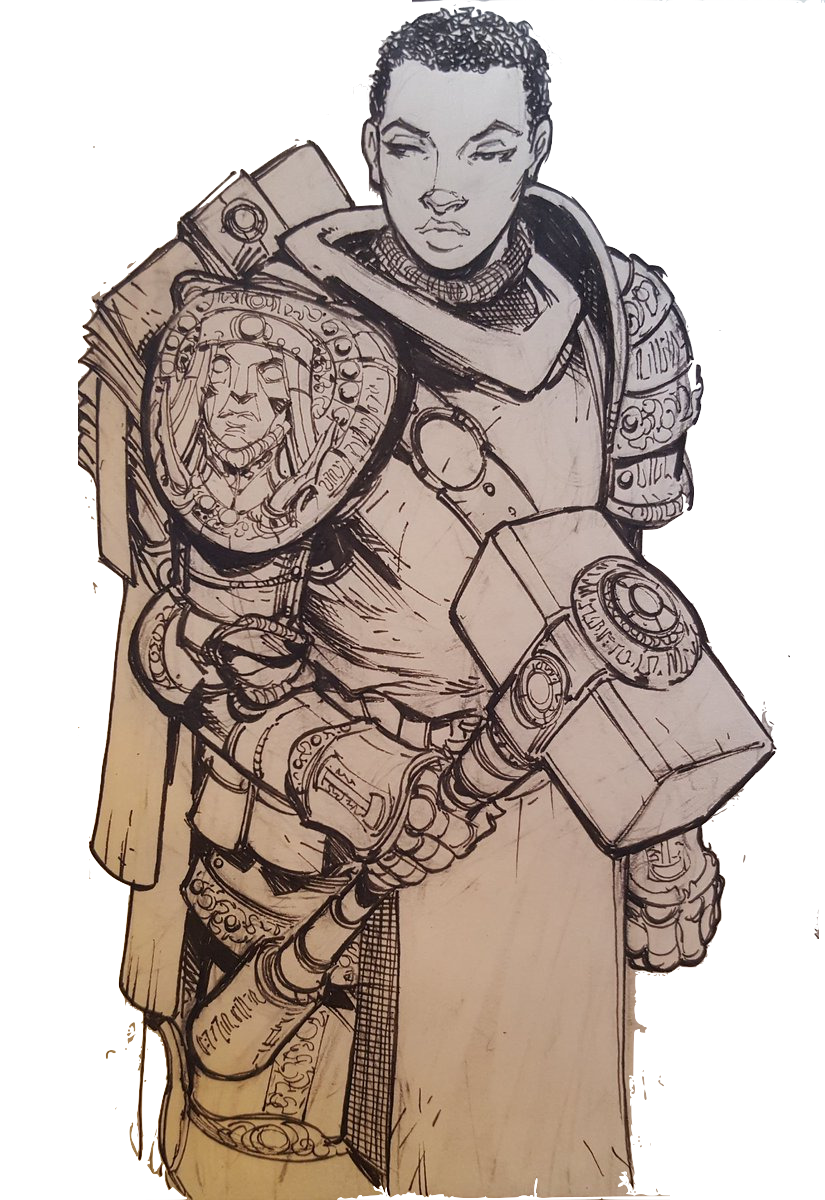
\includegraphics[width=\textwidth]{img/paladin-2.png}
\end{Figure}
    
\end{multicols*}

    